\chapter{Clustering Analysis}

The econometric model used in this paper assumes homogeneous behavior among financial institutions. However, it is possible that there are different groups of banks with distinct characteristics and behaviors. \citeonline{farneBanksBusinessModels2021} propose a cluster analysis using the factorial k-means method to identify different business models among banks and suggest this as a way to analyse an "increasingly diverse banking industry landscape". \citeonline{atheyMachineLearningMethods2019} more generally suggest "use cluster membership as a way to organize the sample into types of units that may receive different exposures to treatments."

Our objective is to use the clustering analysis to identify groups of financial institutions with similar characteristics and behaviors, and then the econometric model can be applied to each group separately, allowing for a more precise understanding of the dynamics of the banking industry.

The k-means clustering algorithm is a widely used method for partitioning a dataset into $K$ distinct clusters based on the similarity of the data points. Given a set of observations $X_i$ defined by the balance sheet accounts divided by total assets  of the $i$-th financial institution, the goal is partition the feature space into $K$ subspaces \cite{atheyMachineLearningMethods2019}. 


\section{Data preparation}

The data used are monthly financial statement accounts of financial institutions obtained from the \citeonline{financialdata}. It covers the period from 2010 to 2024 and includes 206 accounts. Most of those accounts are very specific for some institutions, so the data with more than 30\% of missing values were excluded, resulting in 56 accounts. The sample was limited to financial institutions with at least 1 billion reais in credit operations. Since the data is monthly, the value of each variable is the average of the 12 months of the year, institutions that didn't have data for all 12 months were excluded of that year. Then, each variable is divided by the total assets of that institution at that year to make the data comparable across institutions of different sizes. Finally, each variable is standarized with mean zero and standard deviation one.

The database has 3210 observations (financial institution per year) and 56 variables. To exclude outliers of each year, we used the Principal Component Analysis (PCA) method. It was calculated the first 4 principal components for each year and the observations with values higher than 4 standard deviations in any of the first 4 principal components were excluded. This resulted in the final database with 3210 observations.

\section{Factorial K-means (FKM)}

The Factorial K-means was first proposed by \citeonline{vichiFactorialKmeansAnalysis2001} to add dimensionality reduction to the classic K-means.

The k-means algorithm aims to partition the data into $K$ clusters by minimizing the within-cluster sum of squares (WCSS), which is defined as the sum of the squared distances between each data point and the centroid of its assigned cluster. The algorithm starts with an initial set of $K$ centroids, which can be randomly selected from the data points or initialized using a specific method. Then, it iteratively assigns each data point to the nearest centroid and updates the centroids by calculating the mean of the data points in each cluster. This process continues until convergence, which occurs when the assignments no longer change or when a maximum number of iterations is reached.

In the K-means model, given a dataset $X_{N \times P}$ of $N$ banks and $P$ variables and the centroid matrix $Z_{K \times P}$ with $K$ clusters, the objective is to find the the partition $U_{N \times K}$ that minimizes the within clusters sum of squares (WCSS):

\begin{equation}
    \min_{U,Z} \sum_{i=1}^N \sum_{j=1}^K u_{ij} \Vert x_i -z_j \Vert ^2
\end{equation}

$u_{i,j}$ is a dummy variable that equals 1 if bank $i$ belonggs to cluster $j$ and 0 otherwise.

FKM adds a projection matrix $V_{P \times d}$ to reduce the original variables $P$ to the factors $d < P$. 

Factors are linear combinations of the original variable set subject to the restriction they are orthogonal to each other. Each factor is a vector of loadings for each original variable, loadings range between 1 and -1 and measure the strength and direction of the relationship between the original variable (e.g., Demand Deposits) and the latent dimension (Factor 1). The higher the absolute loading value, the greater the importance of the variable to explain the factor. The optimization problem is to minimize the euclidian distance in the projected space:

\begin{equation}
    \begin{aligned}
        \min_{U,V,Z} \sum_{i=1}^N \sum_{j=1}^K u_{ij} \Vert V^T x_i -z_j \Vert ^2 \\
        \text{s.t.} V^T V = I_d
    \end{aligned}
\end{equation}

$V^T x_i$ is the projected point on the factors space.

The FKM algorithm solves this equation using the Alternating Least Squares (ALS) method. It alternates between two steps, it fixes the projection matrix $V$ to find the best $U$ and $Z$ (which is equivalent to the classic K-means) and it fixes $U$ and $Z$ to find the best $V$. The process is repeated until the WCSS stops decreasing.

The number of clusters and factors is exogenous to the model and there is no single method to help define it. \citeonline{farneBanksBusinessModels2021} use the Hartingan metric witch compares the $WCSS$ using $K$ clusters and $K+1$ clusters.
$$H(k) = \left( \frac{WCSS_k}{WCSS_{k+1}} - 1 \right) \cdot (N - k - 1)$$
The ideal $K$ is defined as the point where the relative reduction in $WCSS$ ceases to be statistically significant enough to justify the loss of degrees of freedom. Hartigan mathematically requires that $WCSS_{k+1} \le WCSS_k$. It assumes the same space is being partitioned. However, in FKM, the factor matrix changes with each $k$. When moving to $k+1$, the algorithm creates an entirely new space, which can result in $WCSS_{k+1} > WCSS_k$. 

Another method is the Average Silhouette Width (ASW), it compares the average distance of each bank to all banks in the nearest cluster $b_i$ with the average distance of each bank to all the banks in the same cluster $a_i$. A larger silhouette means the clusters are more separated.
$$s = \sum_{i=1}^N \frac{b_i - a_i}{\max(a_i, b_i)}$$

In this study, the method used is the ASW

\begin{table}[!ht]
    \centering
\begin{tabular}{@{}ccccc@{}}
                                    \cmidrule(l){2-5}
                                    &  & \multicolumn{3}{c}{Number of factors} \\ \cmidrule(l){2-5}
                                    &  & 2 & 3 & 4 \\
\multirow{4}{*}{\rotatebox[origin=c]{90}{Clusters}}& 3 & 0.128 &  &  \\
                                    & 4 & 0.075 & 0.15 &  \\
                                    & 5 & 0.02 & 0.063 & 0.097 \\
                                    & 6 & 0.017 & 0.045 & 0.052 \\ \cmidrule(l){2-5} 
\end{tabular}
    \caption{Average Silhouette Width (ASW)}
\end{table}



%\section{Principal Component Analysis (PCA)}

%This method is a multivariate statistical technique for unsupervised learning to reduce the dimensionality of the data while retaining as much information as possible. It does this by finding the directions (principal components) that maximizes the variance explained in the data, and then projecting the data onto these directions. In other perspective, the first principal component is the linear regression that minimizes the orthogonal distance between the data points and the regression line and the other components are defined in the same way but with the restriction that they are orthogonal to the previous components. Ther result is a new set of variables (the principal components) that are uncorrelated and ordered by the amount of variance they explain in the data. The first few principal components can be used to represent the data in a lower-dimensional space, which can be useful for visualization and clustering.

%\citeonline{IntroductionStatisticalLearning2023} define the first principal component as regression line that "minimizes of squared perpendicular distances between each point and the line". It is similar to OLS regression, but instead of minimizing the vertical distances between the data points and the regression line, it minimizes the orthogonal distances. Each subsequent principal component is defined in the same way but with the restriction that it is orthogonal to all previous components. The result is a new set of variables (the principal components) that are uncorrelated and ordered by the amount of variance they explain in the data.

%Each principal component has a proprtion of the total variance in the data that it explains, which is called the explained variance ratio. The explained variance ratio is the proportion of the total variance in the data that is explained by each principal component, it can be used to determine how many principal components to retain in order to capture a certain percentage of the variance in the data.

%The PCA was used in this study in two different ways: first to exclude outliers and then to reduce the dimensionality of the data before applying the k-means clustering algorithm. To exclude outliers, the database was separated for each year and the variables were normalized to mean zero and standard deviation one. Then the first 4 principal components were calculated for each year and the explained variance ratio of the first four components was very close to 50\% on each year. The observations with values higher than 4 standard deviations in any of the first 4 principal components were excluded. This resulted in the final database with 3150 observations.


%After excluding outliers, the PCA was used to address the high dimensionality of the data. \citeonline{steinbachChallengesClusteringHigh2004} explain that in high dimensionality, the distance between points becomes less meaningful as they become relatively uniform, which can lead to less precise clustering results. In other words, if the financial institutions have many variables (balance sheet accounts), the difference between them become less meaningful and the clusters may not be well defined. The PCA method is an alternative to reduce the dimensionality of the data while retaining as much information as possible.

%To reduce the dimensionality of the data, the data was standarized with mean zero and standard deviation one without the year segmentation. The PCA method needs to specify the number of principal components (PCs) to retain, which can be determined by looking at the explained variance ratio. The k-means algorithm also needs to specify the number of clusters $K$, one way to determine the optimal number of clusters is by calculating the silhouette score, which measures how well each data point fits within its assigned cluster compared to other clusters. The silhouette score ranges from -1 to 1, where a score close to 1 indicates that the data point is well matched to its own cluster and poorly matched to neighboring clusters, while a score close to -1 indicates that the data point is poorly matched to its own cluster and may be better assigned to a neighboring cluster.

%The number of principal components retained may affect the clusteing results, so the strategy used here is to find the for each $K$ number of clusters the number of principal components that maximizes the silhouette score. The optimal number of clusters is then determined by looking at the silhouette scores for different values of $K$ and selecting the one that yields the highest score. The results are shown in Figure \ref{fig:PCA_optimization}. The chosen $K$ was 5 and the number of principal components retained was 14, which explains 80\% of the variance in the data. The silhouette score for this configuration was 0.19, which indicates that the clusters are reasonably well defined, but there is still some overlap between them. The data has 56 variables that the PCA reduced to 14 principal components.



\section{Cluster Results}

The three factors found were named based on the variables with higher absolute loading values:

Factor 1 (Core deposits) indicates institutions with high liquidity through core deposits, high fixed assets but less diversified operations with low investments and interbank deposits.

Factor 2 (Onlending funding) shows higher credit volume and high Borrowings and onlendings which represents funds raised from other intitutions (development banks, international development agencies).The cost of funds is also higher 

Factor 3 (High risk credit) indicates higher risk intitutions more dependent on credit and fee incomes. Low cost of funds may be a consequence of companies that raise funds with equity and securitization strategies.

The clusters were then defined based on the combination of values on each centroid, based on these values we can see the main characteristics that differentiate business models. The differences between the clusters are mostly based on type of funding and revenue sources. The cluster centroids are shown in table \ref{tab:cluster_centroids}.

\begin{table}[!ht]
    \centering
\begin{tabular}{@{}ccccc@{}}
                                    \cmidrule(l){3-5}
                                    &  & \multicolumn{3}{c}{Factor} \\ \cmidrule(l){3-5}
                                    &  & 1 & 2 & 3 \\
\multirow{4}{*}{\rotatebox[origin=c]{90}{Cluster}}& 1 & 0.107 & -0.093 & -0.234 \\
                                    & 2 & -0.217 & 0.199 &-0.163 \\
                                    & 3 & -0.337 & -0.019 & 1.062 \\
                                    & 4 & 0.704 & -0.265 & -0.128 \\ \cmidrule(l){2-5} 
\end{tabular}
    \caption{Cluster Centroids}
    \label{tab:cluster_centroids}
\end{table}


Cluster 1 (Specialized multi-service banks focused on consumer credit) has the higher proportion of on demand deposits, time deposits, and fixed asset intensity among the four groups, which indicates that this cluster, as well as the second highest concentration of credit operations. This combination characterizes banks with a strong specialization in consumer credit that also possess full access to banking funding sources, structurally distinguishing them from the pure finance companies in Cluster 3.

Cluster 2 (Diversified Conglomerates and Wholesale Players with a Strong Local Presence) comprises the country's five largest banks (Banco do Brasil, Bradesco, Itaú Unibanco, Santander, Caixa Econômica Federal), foreign investment and wholesale banks with substantial local operations (J.P. Morgan, Citibank, Credit Suisse, BNP Paribas, Goldman Sachs, BofA Merrill Lynch, UBS), manufacturer-affiliated captive finance companies (John Deere, Caterpillar, CNH Industrial, Mercedes-Benz, Scania, Toyota, PACCAR, Komatsu), regional development banks, and various niche SCDs/fintechs. In terms of gross averages, this cluster shows the lowest (or near-lowest) values across virtually all line items simultaneously—a pattern consistent with large balance sheets diversified across multiple activities (lending, treasury, foreign exchange, services), which proportionally dilutes each individual ratio. The only notable exception is the highest average for repurchase agreements among the four clusters.

Cluster 3 (Finance Companies) has institutions with operations mostly concentrated in credit, 75\% of this cluster has no demand deposits which shows that this cluster has a high concentration of finance companies. This cluster also has high provisions which indicates high-risk portfolios and the highest level of funding via interbank deposits among the four clusters reflecting reliance on the interbank market as a more expensive alternative funding source due to regulatory restrictions on accepting deposits from the general public. Most of the institutions on this cluster are finance companies.

Cluster 4 (Wholesale and Foreign Banks) is the smallest cluster, composed of institutions with a large cash buffer and securities portfolio. It is a strategy typical of Securities holding banks and a large part of this cluster is formed of wholesale foreign banks like Rabobank, Credit Suisse, ING and Deutsche Bank. The cluster profile is dominated by foreign exchange portfolios (on average, 8.2\% of the total asset, approximately 15 times the Cluster 2 average) and foreign exchange income (also the highest among the clusters), as well as higher levels of securities, interbank investments, and other receivables, consistent with low local credit intermediation and a focus on treasury and foreign exchange operations. %The average proportion of loan and on-lending liabilities is highest among the four clusters, which may differ from the factor 2 low score (-0.265), these insitutions rely heavily on loans raised from their overseas parent companies.

Figure \ref{fig:cluster_discrimination} illustrates the profile of each cluster based on the most discriminating balance sheet accounts, identified from the Factorial K-Means model with the highest loadings in absolute value (the account obligations for borrowings and onlendings under liabilities is divided into three groups: domestic borrowings, domestic on-lendings, and the sum of the liabilities from foreign borrowings and foreign on-lendings). For each account, a z-score was calculated for each individual institution relative to the mean and standard deviation of the full sample, the values represent the distance in standard deviations from the overall sample mean. Subsequently, these standardized scores were aggregated using a simple average within each cluster.


\begin{figure}[h!] % [h!] força a posição, pode ser [!htb]
    \centering
    \includegraphics[width=0.7\textwidth]{cluster_discriminanting_variables.png} % Ajusta largura
    \caption{Comparative profile based on the most discriminating variables}
    \label{fig:cluster_discrimination}
\end{figure}

We can see from Figure \ref{fig:cluster_discrimination} that Cluster 3 is the one with the most concentrated operations in credit and the largest volume of provisions, indicating a higher risk. Also is more dependent on expensive funding sources like interbank deposits and on-lending. Cluster 4 has high volume of foreign operations indicating the presence of foreign banks. Clusters 1 and 2 have a more balanced profile, but cluster 2 has the highest concentration of domestic intitutional funding and a lower concentration of credit operations than cluster 1, which indicates a more diversified business model while cluster 1 has a more traditional retail bank model.


Figure \ref{fig:cluster_risk_composition} illustrates the composition of the credit portfolio by risk level for each cluster. Cluster 3 is the one with the highest proportion of high-risk credit operations, Cluster 4 has the portfolio with the lowest risk but has the lower proportion of credit operations over total assets.

\begin{figure}[h!] % [h!] força a posição, pode ser [!htb]
    \centering
    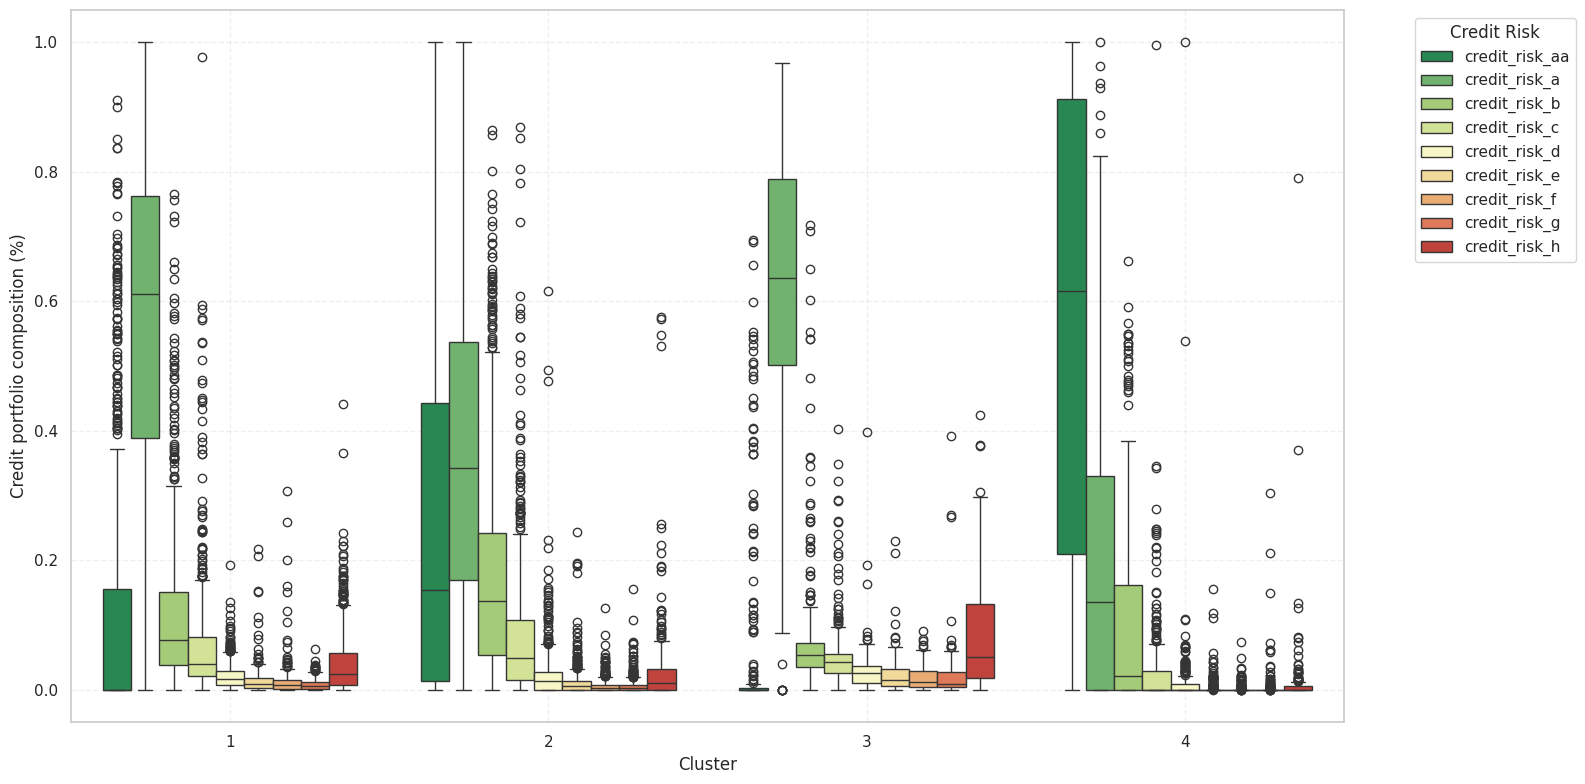
\includegraphics[width=0.8\textwidth]{cluster_risk_composition.png} % Ajusta largura
    \caption{Composition of Credit Portfolio by Risk Level for each cluster}
    \label{fig:cluster_risk_composition}
\end{figure}



%Before 2018, one category of financial institutions known as "sociedade de crédito ao microempreendedor e à Empresa de Pequeno Porte" (SCMEPP) did not have it's financial statements disclosed, this changed after a Central Bank's resolution that made the disclosure mandatory \cite{resolucao_bcb}. So in the the data we can see a signifiant increase in the number of institutions in cluster 4 after 2018, which is the cluster that contains most of the SCMEPPs. Also in 2018, the, it was created the "sociedade de crédito direto" (SCD), which is a new type of financial institution that operates exclusively through digital platforms and has a more flexible regulatory framework \cite{resolucao_bcb2}. The SCDs start appearing in the data in 2019 and are only 52 institutions, but they are growing rapidly wth only one in 2019, 34 in 2023 and 39 in 2024.

%Cluster 3 was empty until 2020 and is composed by SCDs, it represents a very small group of institutions and may be a result of changes in regulation and the emergence of new types of financial institutions. 

%The cluster 0 is the most stable over time, with a consistent number of institutions throughout the years. Banks are 78\% of the institutions in this cluster, and they are the largest financial institutions in terms of total assets. Considering the total volume of credit operations in each year, the institutions in cluster 0 are responsible for around 84\% to 91\% of the total credit operations in each year of the data. Only the  top 6 institutions in terms of credit operations are responsible for around 70\% of the total credit operations in each year and all of them are in cluster 0. But even excluding the top 6 institutions, cluster 0 still has the biggest share of credit aoperations as shown in Figure \ref{fig:cluster_mkshare}. This indicates that cluster 0 is the most dominant cluster in terms of credit operations, even when excluding the largest institutions. The other clusters have a much smaller share of credit operations, with cluster 2 being the second largest but still significantly smaller than cluster 0.








%Cluster 1 is similar to cluster 0 in terms of risk exposure, but it has a much higher ratio of administrative expense to total assets and has smaller institutions. This indicates that cluster 1 may be less efficient 

%Cluster 2 is the second biggest cluster and is composed by Institutions more specialized in credit, with a higher ratio of credit operations over total assets. The cluster is composed mostly by banks, but also has a significant share of finance companies. 

%Cluster 4 is the one which absorbed most of the SCMEPPs after 2018, it is composed mostly by finance companies and has a higher share of credit operations over total assets than cluster 0, but lower than cluster 2. It has more risky credit operations classified as "level h" and "level f" in the data, which are operations with higher risk of default. It also has the higher ratio of credit provisions over credit operations.




